\documentclass[11pt,a4paper]{article}
\usepackage[margin=25mm]{geometry}
\usepackage{amsmath,amssymb,graphicx,booktabs,float,hyperref}
\usepackage{microtype}
\graphicspath{{../figures/}{../stage2_D_runs/20261105T132543802032Z/figures/}}
\title{Perpetual American Put\\\large A finite-difference obstacle problem}
\author{Coursework team: names and individual contributions to be completed}
\date{Technical draft, 6 November 2026}
\begin{document}\maketitle
\begin{abstract}
We calculate the value and exercise threshold of a perpetual American put using a monotone finite-difference linear complementarity problem and policy iteration. The constant-volatility benchmark validates both the price and the threshold against an analytic solution. A local-volatility case is examined with four meshes, two refined references, three truncated domains, and independent continuous shooting and collocation calculations. For the finest study grid, the maximum price difference to the primary reference is $0.004604$ on $[0,600]$. The price at $S=100$ changes by $0.234265$ when the boundary moves from $400$ to $600$. A small algebraic residual therefore coexists with material truncation sensitivity. This is a technical draft. Student review, authorship, and formal course audit remain to be completed.
\end{abstract}
\tableofcontents
\clearpage
%%%%%%%%%%%%%%
\section{Background and model}\label{sec:model}
A perpetual American put gives the holder the right to sell an asset for $K$ at any stopping time. Let $S$ be its price, $r$ the discount rate, $q$ the dividend yield, and $\sigma(S)$ the local volatility. The immediate exercise payoff is $\psi(S)=(K-S)^+$. In the risk-neutral model, continuation has differential operator
\begin{equation}\label{eq:operator}
\mathcal L V = \tfrac12\sigma(S)^2S^2V''+(r-q)SV'-rV.
\end{equation}
The value satisfies the obstacle problem
\begin{equation}\label{eq:obstacle}
\min\{-\mathcal L V,\,V-\psi\}=0,\qquad S>0,
\end{equation}
with $V(0)=K$ and $V(S)\to0$ as $S\to\infty$. The course problem statement provides the benchmark and scope \cite{pack,brief}. The continuation equation is a second-order ODE because there is one state variable and no expiry time. The complementarity formulation also illustrates the obstacle problems arising in elliptic PDEs. In the exercise region the value equals the payoff, while in the continuation region the differential equation holds. Value matching and smooth fit at the exercise threshold $S^*$ are
\begin{equation}\label{eq:smoothfit}
V(S^*)=K-S^*,\qquad V'(S^*)=-1.
\end{equation}
All experiments use $K=100$ and $r=0.05$. The first stage uses $q=0$ and constant $\sigma=0.20$. The second uses $q=0.02$ and
\begin{equation}\label{eq:localvol}
\sigma(S)=0.20\left[1+0.35\tanh\left(\frac{\log(S/100)}{0.40}\right)\right].
\end{equation}
The local volatility lies between $0.13$ and $0.27$. The calculation imposes the left boundary directly without evaluating the logarithm at zero.
\clearpage
%%%%%%%%%%%%%%
\section{Discretisation and policy iteration}\label{sec:methods}
For a uniform mesh $S_i=ih$ on $[0,L]$, write $d_i=\sigma(S_i)^2S_i^2/2$ and $b_i=(r-q)S_i$. The monotone discretisation of $-\mathcal L$ has coefficients
\begin{equation}\label{eq:stencil}
\ell_i=-d_i/h^2-b_i^-/h,\quad c_i=2d_i/h^2+|b_i|/h+r,\quad u_i=-d_i/h^2-b_i^+/h,
\end{equation}
where $b_i^+=\max(b_i,0)$ and $b_i^-=\max(-b_i,0)$. The off-diagonal entries are nonpositive and the full row dominance margin is $r>0$. Contributions of prescribed endpoints move to the right-hand side $f$. The unknown interior vector $v$ obeys
\begin{equation}\label{eq:lcp}
a=Av-f\ge0,\quad g=v-\psi\ge0,\quad \min(a,g)=0.
\end{equation}
Policy iteration for American option problems is discussed in \cite{policy}. Policy iteration starts from the payoff. Each iteration chooses the exercise row when $g_i<a_i$ and otherwise keeps the continuation row. A banded direct solve yields the next iterate. The stopping residual is $\rho=\|\min(a,g)\|_\infty$. Exact ties choose continuation. A repeated policy can terminate at a floating-point residual floor, which is separately recorded and does not imply the requested tolerance was met. The initial iterate, iteration count, actual residual and termination status are stored with each calculation.

The exercise threshold is the last node in the contact interval connected to zero, with $|V_i-\psi_i|\le10^{-7}$ and $S_i<K$. The artificial right endpoint is excluded. The following node describes the discrete transition. This interval is not asserted to enclose the continuous threshold.
\clearpage
%%%%%%%%%%%%%%
\section{Verification design}\label{sec:verification}
The first benchmark has an analytic continuation solution. Substituting $V(S)=CS^\lambda$ into the continuation equation gives the negative root $\lambda=-2.5$, whence
\begin{equation}\label{eq:exact}
S^*=500/7,\qquad V(S)=\begin{cases}100-S,&S\le S^*,\\(100-S^*)(S/S^*)^{-2.5},&S>S^*.\end{cases}
\end{equation}
The Stage 1 mesh study uses the analytic value at $L=400$, removing the artificial endpoint error from this comparison. We measure the maximum nodal price error and the absolute threshold error. The discrete $L^2$ norm is also available in the saved tables.

Stage 2 uses the prescribed zero value at $L$. The mesh study fixes $L=600$ and compares nested nodes against $h=1/128$. The second reference at $h=1/256$ measures sensitivity to the choice of reference. The domain study fixes $h=0.0625$ and compares $L=300,400,600$. The recorded componentwise minima, complementarity residual, bounds, monotonicity, convexity and contact connectivity support each calculation.

An independent ODE shooting method integrates backward from the zero endpoint and determines the threshold from smooth fit. A second implementation solves a transformed free-boundary problem by adaptive collocation with the threshold as an unknown parameter. These checks share the continuous model and boundary conditions while using different numerical methods. An exhaustive active-set enumeration on small grids independently checks the policy solver for the assembled matrix. The repository contains the actual inputs, raw arrays, diagnostics and tests.
\clearpage
%%%%%%%%%%%%%%
\section{Constant-volatility results}\label{sec:stage1}
Table~\ref{tab:stage1} records the four mesh levels. The observed price order is about one, as expected for the first-order drift stencil. A log-log fit over all four levels gives $p\approx0.996$. The boundary error is nonmonotone because the threshold is extracted from grid nodes. The smooth-fit diagnostic is supporting evidence alongside the full price and threshold comparisons.
\begin{table}[H]\centering\caption{Stage 1 on $[0,400]$ with analytic right boundary.}\label{tab:stage1}
\begin{tabular}{rrrrr}\toprule
$h$ & max price error & threshold & threshold error & LCP residual \\\midrule
0.5 & 0.058473 & 71.5000 & 0.071429 & $2.11\cdot10^{-11}$ \\
0.25 & 0.029348 & 71.2500 & 0.178571 & $4.86\cdot10^{-11}$ \\
0.125 & 0.014735 & 71.3750 & 0.053571 & $2.92\cdot10^{-11}$ \\
0.0625 & 0.007363 & 71.4375 & 0.008929 & $1.16\cdot10^{-10}$ \\\bottomrule
\end{tabular}\end{table}
The requested tolerance was $10^{-8}$ for all four rows. The stored values are from \path{results/stage1_convergence.csv}. The separate Stage 1 script may reproduce slightly different last digits across platforms. Figure~\ref{fig:convergence} shows the two price-refinement studies.
\begin{figure}[H]\centering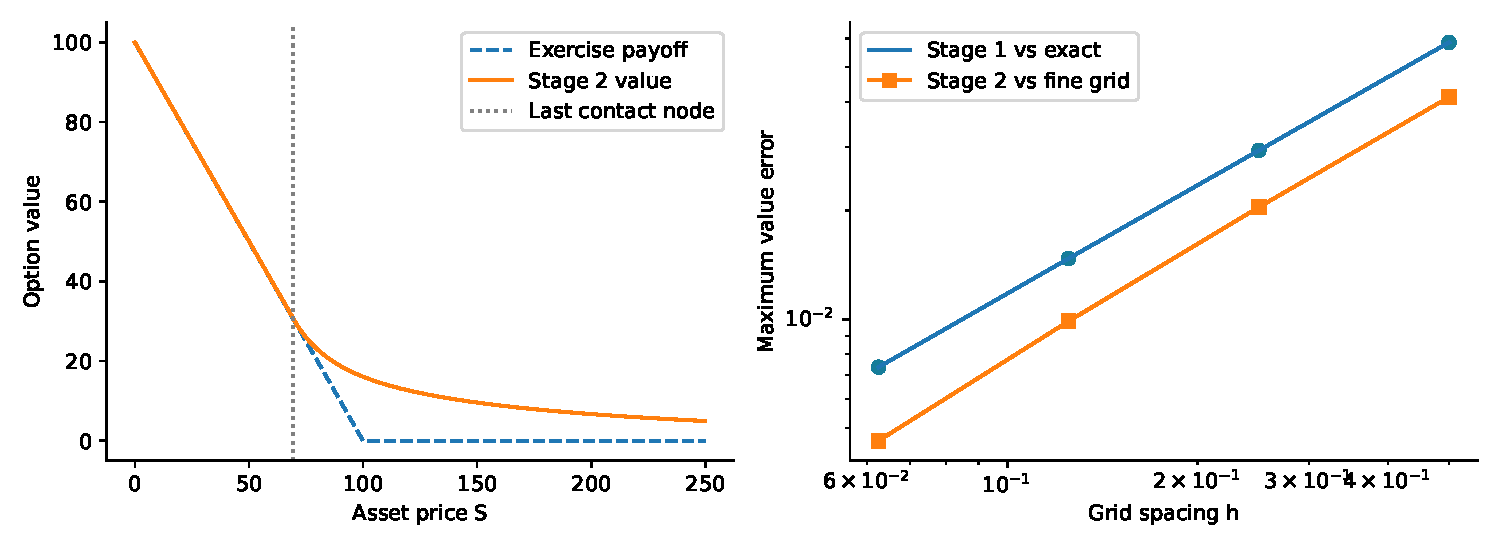
\includegraphics[width=.88\textwidth]{value_and_convergence.pdf}\caption{Price profiles and maximum-norm mesh differences.}\label{fig:convergence}\end{figure}
\clearpage
%%%%%%%%%%%%%%
\section{Local volatility and reference sensitivity}\label{sec:stage2}
Table~\ref{tab:stage2} compares each mesh with the $h=1/128$ reference at coincident nodes. The maximum difference of the two references is $3.2843\cdot10^{-4}$, about $7.13\%$ of the finest study difference. The reference is therefore useful for the qualitative rate and contributes a visible bias to the finest measured difference. The fitted log-log order over the four displayed differences is about $1.054$. Against the independently integrated ODE solution, the fitted order is about $0.998$.
\begin{table}[H]\centering\caption{Stage 2 refinement on $[0,600]$.}\label{tab:stage2}
\begin{tabular}{rrrrr}\toprule
$h$ & max difference & pairwise order & contact node & residual \\\midrule
0.5 & 0.041218 & -- & 69.0000 & $4.70\cdot10^{-11}$ \\
0.25 & 0.020437 & 1.012 & 69.2500 & $3.87\cdot10^{-11}$ \\
0.125 & 0.009875 & 1.049 & 69.2500 & $1.76\cdot10^{-10}$ \\
0.0625 & 0.004604 & 1.101 & 69.2500 & $9.56\cdot10^{-10}$ \\\bottomrule
\end{tabular}\end{table}
All study meshes meet the requested $10^{-8}$ residual. The primary and finer reference residuals are $2.98\cdot10^{-8}$ and $1.19\cdot10^{-7}$, respectively, and terminate at a recorded floating-point floor. Repeating the finest reference with a tighter request gives the same stored vector, which measures tolerance sensitivity but does not establish a forward-error bound. Contact-node agreement between the references remains subject to the chosen classification tolerance.
\clearpage
%%%%%%%%%%%%%%
\section{Domain truncation and continuous checks}\label{sec:domain}
At fixed $h=0.0625$, the three truncated domains give the values in Table~\ref{tab:domain}. The shooting and collocation results agree to better than $10^{-6}$ at each endpoint location. At $L=600$, collocation gives $S^*=69.26448256$ and $V(100)=16.06007591$ for the finite-domain problem. These independent continuous checks are recorded in \path{results/independent_audit/collocation.json}.
\begin{table}[H]\centering\caption{Fixed-mesh domain comparison and continuous collocation.}\label{tab:domain}
\begin{tabular}{rrrrr}\toprule
$L$ & $V_h(100)$ & $V_h(200)$ & contact node & collocation $V(100)$\\\midrule
300 & 15.456044 & 4.552002 & 69.6875 & 15.451228 \\
400 & 15.831017 & 5.871201 & 69.4375 & 15.825975 \\
600 & 16.065282 & 6.691671 & 69.2500 & 16.060076 \\\bottomrule
\end{tabular}\end{table}
The change in $V_h(100)$ between $L=400$ and $L=600$ is $0.234265$, materially greater than the finest mesh comparison in Table~\ref{tab:stage2}. Enlarging the domain and refining a fixed domain address different errors. The largest domain is a comparison baseline and does not provide a certified infinite-domain error bound. Figure~\ref{fig:domain} illustrates the domain sensitivity.
\begin{figure}[H]\centering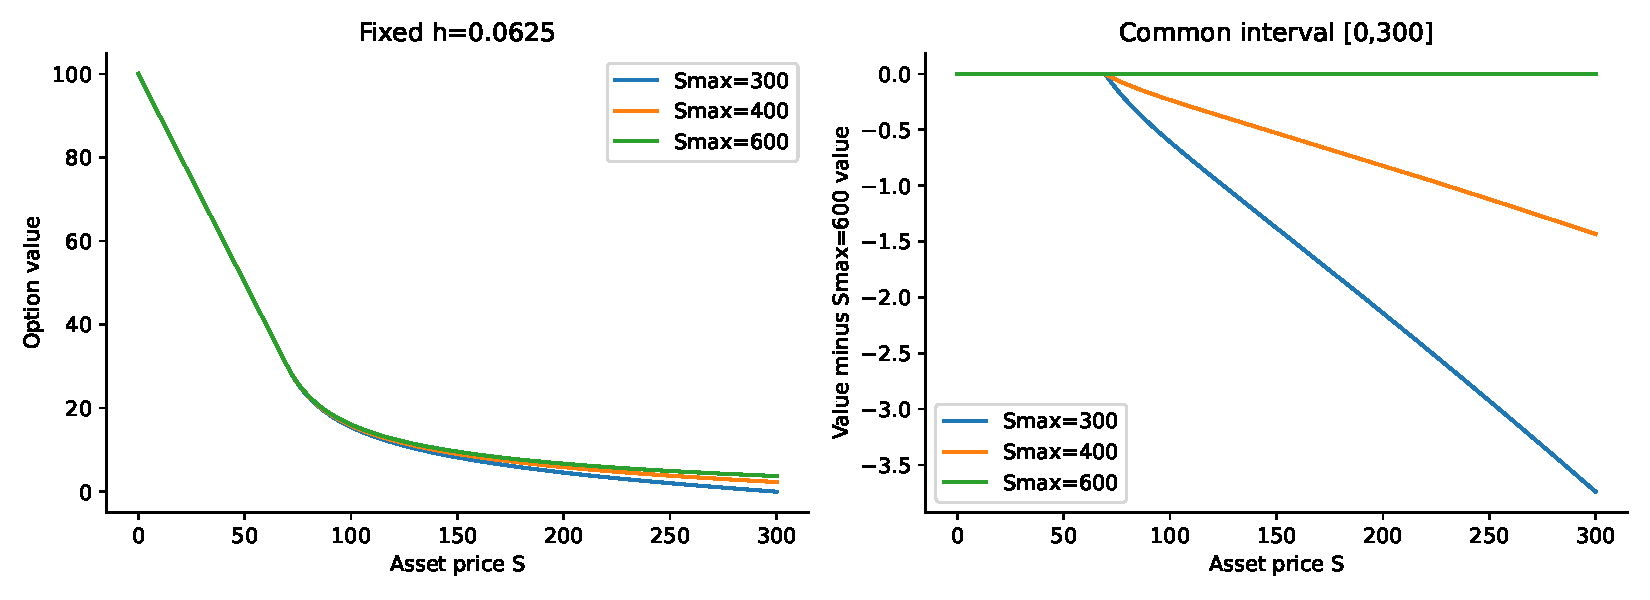
\includegraphics[width=.88\textwidth]{domain_truncation_D.pdf}\caption{Comparison of truncated domains at fixed mesh size.}\label{fig:domain}\end{figure}
\clearpage
%%%%%%%%%%%%%%
\section{Matched solver comparison}\label{sec:solver}
We compare policy iteration and projected SOR on the same Stage 2 matrix, zero endpoint, payoff initial iterate and absolute LCP residual target $10^{-8}$. Projected SOR uses relaxation parameter $\omega=1.2$. On $h=5$ and $2.5$, the methods agree in maximum norm within $4\cdot10^{-8}$. The run records unknowns, iteration counts, residuals and elapsed wall time in \texttt{solver\_comparison.csv} in \texttt{results/independent\_audit/}.

Table~\ref{tab:cost} lists the measured cost. These are single solver calls, including setup, on the recorded machine.
\begin{table}[H]\centering\caption{Matched solver comparison at tolerance $10^{-8}$, with maximum nodal price error relative to shooting.}\label{tab:cost}
\begin{tabular}{rrrrrrr}\toprule
$h$ & unknowns & price error & policy iters & policy sec & PSOR iters & PSOR sec\\\midrule
5 & 119 & 0.4013 & 6 & 0.00044 & 10260 & 1.13 \\
2.5 & 239 & 0.1919 & 12 & 0.00067 & 41073 & 10.77 \\
\bottomrule
\end{tabular}\end{table}

The stored implementation performs projected SOR sweeps in Python, whereas policy iteration delegates its tridiagonal linear systems to compiled SciPy routines. The measured wall-time difference includes that implementation difference and machine effects. A single measured timing is a cost observation and should not be interpreted as a machine-independent algorithmic speedup. The residual target, not an iterate difference, determines termination in both solvers.

The analytic Stage 1 solution, exhaustive tiny-grid active sets and the two continuous Stage 2 calculations supply independent checks of different parts of the chain. The two continuous calculations share the same model transcription, so the parameter and sign checks still matter. The tolerance sweep records identical values under tighter stopping requests on the representative study mesh. The remaining finite-domain bias is not controlled by that sweep.
\clearpage
%%%%%%%%%%%%%%
\section{Conclusions and reproducibility}\label{sec:conclusions}
The monotone LCP solver reproduces the analytic constant-volatility price and approaches the local-volatility fixed-domain solution under mesh refinement. Domain truncation is the dominant observed sensitivity for the chosen endpoints. Further precision for the unbounded model requires a separately justified far-field treatment or larger-domain study. A threshold inferred from contact nodes is limited by mesh and classification tolerance.

From the repository root, install \texttt{american\_put\_project/requirements-dev.txt} and run \texttt{python -m pytest -q}. The working scripts, saved results, independent checks and figure sources are described in the repository README. The staged report data come from the recorded runs and the separate solver comparison. Numerical timings depend on the platform.

AI assisted with modelling, code, experiments, review and drafting. The saved AI-generated prediction records were written before their associated runs and are labelled accordingly. Each student must complete their own predictions and reconciliation as required by the course, reproduce and interrogate the methods, and record actual individual contributions. These human actions and the course's formal five-gate worksheet remain pending. The independent numerical checks reported here are technical evidence for that review.
\begin{thebibliography}{9}
\bibitem{pack} Course materials, \emph{Problem Pack, Project 2}, perpetual American put direction, pp.~8--9.
\bibitem{brief} Course materials, \emph{Project 2 Brief}, pp.~1--4.
\bibitem{policy} C. Reisinger and J. H. Witte, On the use of policy iteration as an easy way of pricing American options, \emph{SIAM Journal on Financial Mathematics} 3 (2012), 459--478, \url{https://doi.org/10.1137/110823328}.
\end{thebibliography}
\end{document}
